\documentclass{article}

\usepackage[utf8]{inputenc}
\usepackage{amsmath, enumitem, url}

% For figures.
% Package float, adds the H option which forces figure placement.
\usepackage{graphicx, float}
\graphicspath{ {./figures/} }

\title{Exploration of End-to-End Verifiable Voting Systems}
\author{Mikhail Skobov and Keyan Pishdadian}
\date{December 2020}

\begin{document}
\maketitle

\section*{Summary}
We present a brief overview of the motivation for and goals of secure electronic voting systems and the most common current techniques used to tackle this problem. The focus of our work is the discussion of one particular solution to the electronic voting problem which leverages split value representations \cite{svr_vote}.

\section{Introduction}
Despite the rapid digitalization of life, most voting systems remain quaintly stuck using dated methods of paper recording and machine-assisted human tabulation. Though attempts have been made in the United States to transition to voting machines and electronic tablets (Direct-Recording Electronics [DRE]), these tools still ultimately rely on the same paper record and manual tallying procedures as a source of truth \cite{ncsl}. These systems do not allow members of the public to personally verify their vote was indeed counted and not manipulated, nor do they allow for a verification of the election outcome itself. As we have seen just this year, these deficiencies pose a serious risk towards maintaining public trust in elections and we will be so bold as to say this puts democracy itself at risk.

The goal of End-to-End Verifiable Voting (E2EVV) systems are to provide an alternative which achieves the following  generally agreed upon requirements \cite{mit}:
\begin{enumerate}
\item
    Individual voters can verify their vote but cannot prove what they voted for (to prevent coercion)
\item
    Individual privacy is maintained
\item
    The election is accurate and votes cannot be altered
\item
    The outcome is verifiable by anyone
\end{enumerate}

Though not often mentioned in the literature, an aspirational requirement is, or at least should be, that the election mechanism is also relatively understandable to the public. This element is crucial in being able to create public trust in any election proof or verification method.

We do not survey the field of E2EVV, but summarize that the existing systems are broadly categorized into three groups based on the core cryptographic component being used to facilitate them: mix-nets, homomorphic encryption, and blind signatures \cite{mit}. There have been production systems for E2EVV though they have not been broadly deployed and trusted to run real elections. The most well known systems found in our research were ElectionGuard \cite{election_guard}\cite{eg_github}, which uses homomorphic encryption, and Helios \cite{helios}, which uses mix-nets. The former of these, ElectionGuard, has actually been used experimentally in at least one real small scale election (alongside traditional paper voting for verification) \cite{newyorker}.

\section{Voting Using Split Value Representations}
We chose to analyze an E2EVV system designed using the mix-net approach \cite{svr_vote}. The main innovation of this paper in comparison to traditional mix-net solutions (such as that used by Helios) is the incorporation of split value representations of votes, the use of primarily computationally efficient modular arithmetic for mixing, and the lack of need for zero-knowledge proofs which simplifies the verification and increases computationally efficiency. Rather than paraphrase the original paper again, the overall protocol is summarized, then some additional details are explained about some aspects of greater importance.

\subsection{Election Steps}
The overall protocol can be broken up into the below steps, note that the Secure Bulletin Board (SBB) discussed below is simply an append-only log that is publicly accessible:
\begin{enumerate}
\item
    Voting - Individual voters submit their votes at a Tablet device.
\item
    Posting of Votes - Tablet devices post encrypted votes to the Secure Bulletin Board (SBB).
\item
    Verification of Postings - Voters can use the SBB to verify their vote was posted.
\item \label{steps:mix}
    Mixing - Votes are obfuscated and shuffled, then posted to the SBB. $2m$ different obfuscations/permutations of the original vote list of posted.
\item \label{steps:proof}
    Proving vote consistency - $m$ out of the total $2m$ lists in step \ref{steps:mix} are partially decrypted in order to allow universal verifiablility of mixing results.
\item \label{steps:outcome}
    Election outcome - The other $m$ of $2m$ lists are fully decrypted and posted to the SBB. This allows anyone to verify and tally the election results.
\end{enumerate}

\subsection{System Overview}
Central to this system is the ``Proof Server", which is a collection of individual servers called ``Mix Servers". The machines in the Proof Server are collectively responsible for mixing votes and posting vote data to the SBB in a way which allows anyone to tally all the votes, ensure that the votes match what was posted by the Tablet devices that voters used to submit their votes, but not be able to tell the identity or vote of any individual voter. An overview of the entire system and all these components is illustrated in Fig. \ref{fig:arch_diagram}.

% To edit see: https://whimsical.com/join/8YfzGdU8o561GspWbuAh5S?invite=bpd6cw4u
\begin{figure}[H]
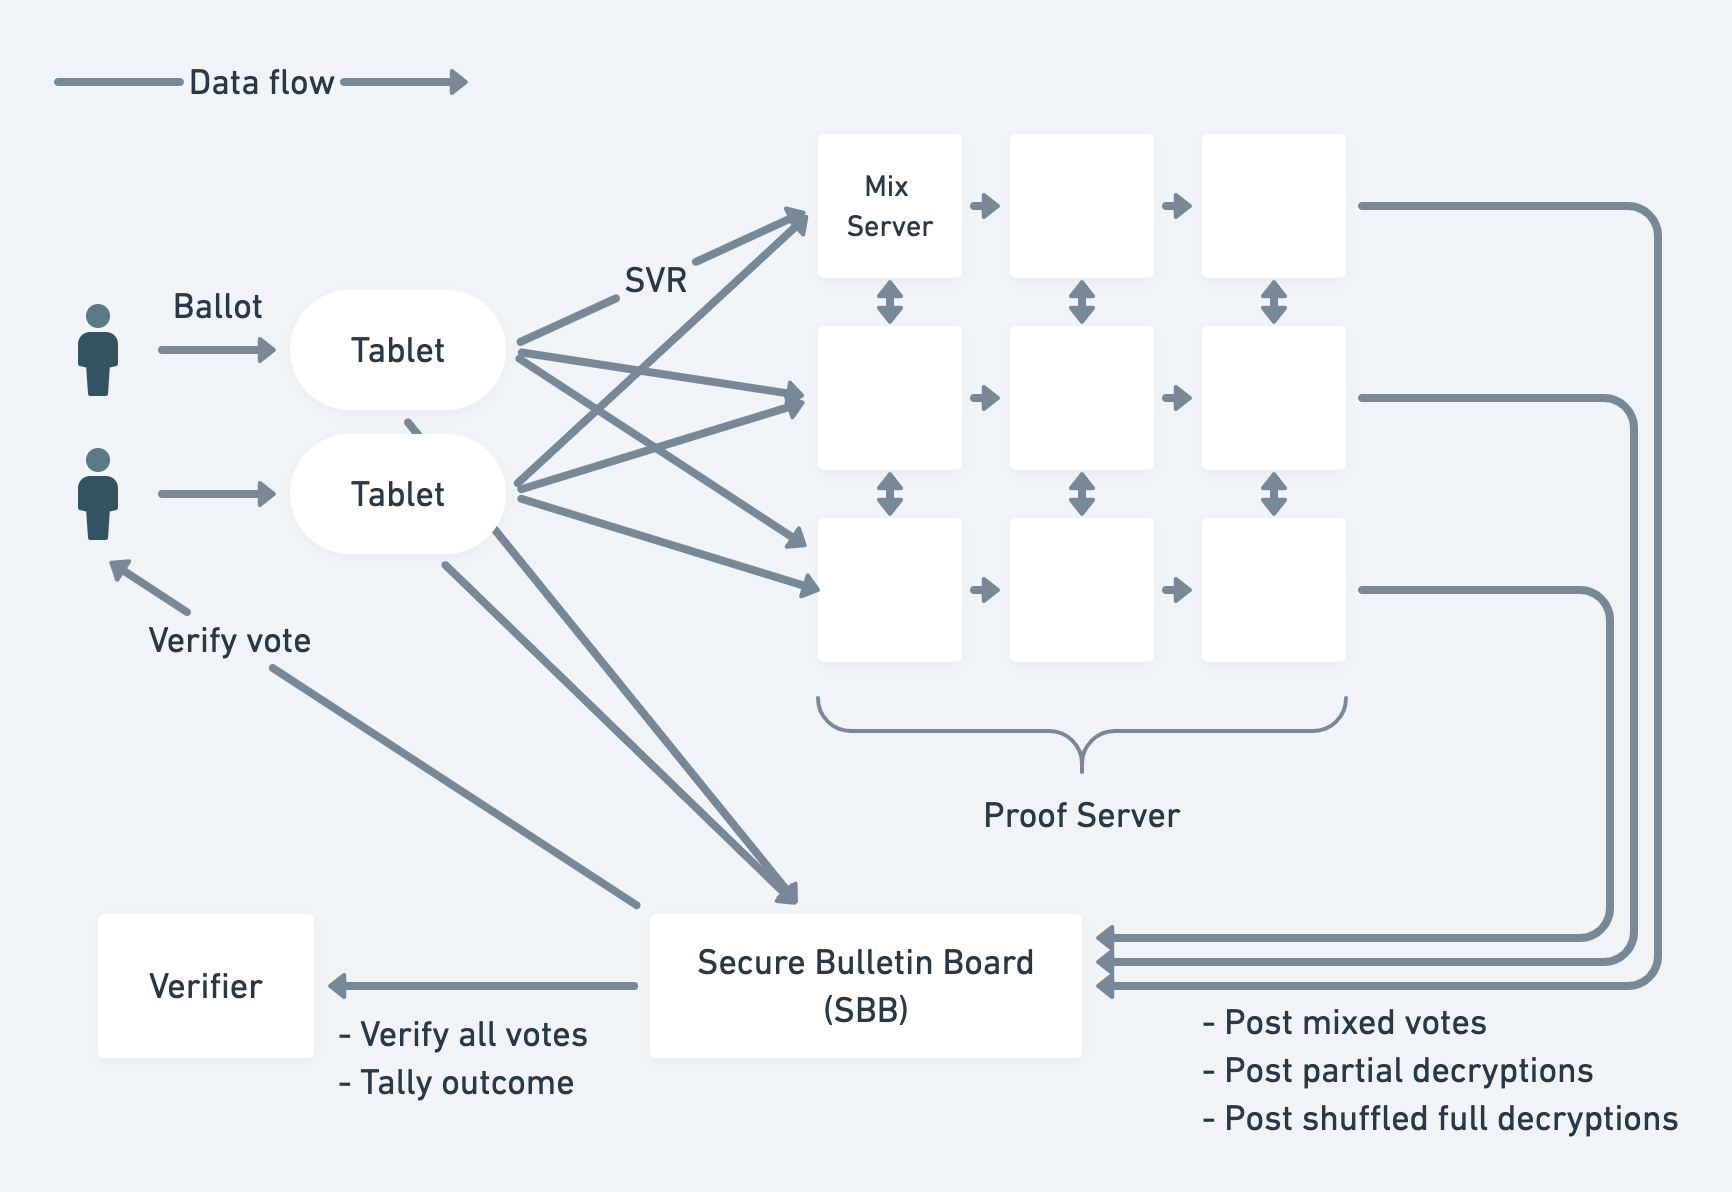
\includegraphics[height=8cm]{arch_diagram}
\centering
\caption{Overview of architecture of the voting system. The Secure Bulletin Board (SBB) is central to the system. Election components write to the append-only SBB meanwhile Voters and Verifiers (any other party) can read data from SBB in order to verify their individual vote was registered or to verify all votes were not altered and compute the final election outcome, respectively. A collection of Mix Servers together make up the Proof Server, which is responsible for mixing split value representations of votes and posting necessary data to the SBB.}
\label{fig:arch_diagram}
\end{figure}

\subsection{Split Value Representations}
Each vote in this system must be represented as an integer $x, 0 \leq x < M$, where $M$ is some integer chosen so there are enough values to represent all possible vote choices. The split value concept used is a form of secret sharing among all the Mix Servers in the Proof Server. A split value representation of a value $x$ is a vector
\begin{equation} \label{eq:svr}
    X = (u, v)
\end{equation}
such that
\begin{equation}
    x = \mathit{VAL}(X) = (u + v) \mbox{ mod } M
\end{equation}

This idea is then extended so that $x$ can be represented with a n-tuple of such vectors. The Proof Server has a configurable number of rows allowed, this row size determines the number of ways each vote is split again. In our example network in Fig. \ref{fig:arch_diagram}, the row size is $3$ so now we would represent the vote $x$ as the vector $(X, Y, Z)$
\begin{equation} \label{eq:comt}
    x = \mathit{VAL}(X) + \mathit{VAL}(Y) + \mathit{VAL}(Z) (\mbox{mod } M)
\end{equation}

The use of an n-tuple to represent the vote $x$ allows the Mix Servers to share the secret among them, performing the mixing operations without any one server knowing the details of an individual vote. That is, row 1 in the Proof Server only ever operates on $(X_1, X_2, \dots, X_n)$ for $n$ votes.

Furthermore, the split value representation using $(u, v)$ for each component of the vote $x$ in Equation \ref{eq:comt} allows for a convenient property where the Proof Server can prove the equivalence of two vote values without revealing the values in their entirety. Only part of the value is needed ($u$ or $v$, but not both) in addition to a value $t$. For example, consider the values $x$ and $y$
\begin{align*} \label{eq:comt}
    x = (u_1 + v_1) \mbox{ mod } M \\
    y = (u_2 + v_2) \mbox{ mod } M \\
    t_u = (u_2 - u_1) \mbox{ mod } M \\
    t_v = (v_1 + v_2) \mbox{ mod } M
\end{align*}
If one is given $(t_u, u_1, u_2)$ or $(t_v, v_1, v_2)$, either is sufficient to validate if $x == y$, but neither triple reveals the true values of $x$ or $y$. This concept is what allows the Proof Server to prove to external parties that the mixed output matches the original cast votes, without revealing what those vote values are. This is important because it maintains privacy for voters and avoids the possibility of vote coercion because voters cannot prove their exact vote value.

Further details on the specifics of the protocol are outside the scope of this report.

\section{Implementation}
The main deliverable of our work is a working implementation of the E2EVV system described above. This implementation runs a simulated election using randomized voters and voting, follows the SBB posting and mixing procedures, and uses the data from SBB to verify votes and compute the election outcome. The code can be found here: \url{https://github.com/keyan/e2e_voting}.

We do not explain specifics of our code here, as it mostly matches the protocol as outlined in the original paper. However, we want to explain several simplifications that were made in order to make implementation feasible within the time constraints and have the focus remain on understanding the cryptographic foundations of the approach rather than on software engineering concerns. Namely,
\begin{enumerate}
\item \label{sim:process}
    Our simulation runs entirely on one machine and one process, while the system in practice would be constructed of multiple physical Tablets, Mix Servers, and a SBB. We use unique class instances to represent each of these entities.
\item
    Related to \ref{sim:process}, the Proof Server is not a collection of servers. Instead we chose to represent the Proof Server as a singleton instance which has a 2D matrix representing the mix-net topology. Rather than Mix Servers using secure communication to pass data during mixing, we pass data freely using instance variables.
\item
    Related to \ref{sim:process}, the SBB is represented as a flat file on disk. Each election entity writes to this file during the election.
\end{enumerate}

\section{Conclusion}
The split-value-representation method provides an appealing solution to the E2EVV problem and its efficient computations, ability to represent complex election races, and relative ease of implementation suggest it could be a viable candidate for use in real life elections. However, there are some deficiencies which we felt were not adequately discussed in the paper. These are:

\begin{enumerate}
\item
    A lack of discussion about handling Tablet device corruption or adversarial manipulation. Being the point of contact between voters and the Proof Server, there was a dearth of evidence that Tablets are robust against tampering despite their critical role in the system.
\item
    A yet inadequate interpretability of the proof and verification stages and computations. Although ease of understanding was purported as one of the main benefits of this system, we found that the verification steps were still difficult to understand without significant effort and providing an intuitive explanation of verification is largely impossible. We believe this is a real barrier to creating practical voting systems because voter trust will be significantly diminished if basic principle of the system cannot be easily explained to a layperson.
\end{enumerate}

Despite this we have great hopes that the future of voting systems will leverage such technology and that our democracy will only be stronger as a result.

\begin{thebibliography}{7}

\bibitem{svr_vote}
Michal Rabin and Ronald Rivest. 2014. Efficient End to End Verifiable Electronic Voting Employing Split Value Representations.

\bibitem{ncsl}
https://www.ncsl.org/research/elections-and-campaigns/voting-equipment.aspx

\bibitem{mit}
Ronald Rivest. 2004. Lecture 17: Introduction to Electronic Voting, lecture notes, 6.837: Advanced Topics in Cryptography, Massachusetts Institute of Technology, delivered April 8 2004.

\bibitem{election_guard}
https://blogs.microsoft.com/on-the-issues/2019/05/06/protecting-democratic-elections-through-secure-verifiable-voting/

\bibitem{eg_github}
https://github.com/microsoft/electionguard

\bibitem{helios}
Ben Adida. 2008. Helios: web-based open-audit voting. In Proceedings of the 17th conference on Security symposium (SS'08). USENIX Association, USA, 335–348.

\bibitem{newyorker}
https://www.newyorker.com/news/the-future-of-democracy/can-our-ballots-be-both-secret-and-secure


\end{thebibliography}
\end{document}
